\documentclass[a4paper]{article}
\usepackage[utf8]{vietnam}
\usepackage[left=3.5cm,right=2.5cm,top=2cm,bottom=2cm]{geometry} 
\setlength{\parindent}{0pt}
\usepackage{graphicx} 
\usepackage{tabularx}
\usepackage{array}
\usepackage{longtable}
\usepackage{multirow}
\usepackage{tocloft}
\usepackage{xcolor}
\usepackage{colortbl} % Required for \arrayrulecolor
\usepackage{tikz} 
\usepackage{scrextend}
\usepackage{makecell}
\usepackage{float}
\changefontsizes{14pt}
\usepackage{enumitem}
\usetikzlibrary{calc}
\usepackage{indentfirst}
\usepackage{ragged2e}
\usepackage[edges]{forest}

\begin{document}
\begin{titlepage}

    \begin{tikzpicture}[remember picture,overlay,inner sep=0,outer sep=0]
        \draw[blue!70!black,line width=4pt] ([xshift=-1.5cm,yshift=-2cm]current page.north east) coordinate (A)--([xshift=1.5cm,yshift=-2cm]current page.north west) coordinate(B)--([xshift=1.5cm,yshift=2cm]current page.south west) coordinate (C)--([xshift=-1.5cm,yshift=2cm]current page.south east) coordinate(D)--cycle;

        \draw ([yshift=0.5cm,xshift=-0.5cm]A)-- ([yshift=0.5cm,xshift=0.5cm]B)--
        ([yshift=-0.5cm,xshift=0.5cm]B) --([yshift=-0.5cm,xshift=-0.5cm]B)--([yshift=0.5cm,xshift=-0.5cm]C)--([yshift=0.5cm,xshift=0.5cm]C)--([yshift=-0.5cm,xshift=0.5cm]C)-- ([yshift=-0.5cm,xshift=-0.5cm]D)--([yshift=0.5cm,xshift=-0.5cm]D)--([yshift=0.5cm,xshift=0.5cm]D)--([yshift=-0.5cm,xshift=0.5cm]A)--([yshift=-0.5cm,xshift=-0.5cm]A)--([yshift=0.5cm,xshift=-0.5cm]A);


        \draw ([yshift=-0.3cm,xshift=0.3cm]A)-- ([yshift=-0.3cm,xshift=-0.3cm]B)--
        ([yshift=0.3cm,xshift=-0.3cm]B) --([yshift=0.3cm,xshift=0.3cm]B)--([yshift=-0.3cm,xshift=0.3cm]C)--([yshift=-0.3cm,xshift=-0.3cm]C)--([yshift=0.3cm,xshift=-0.3cm]C)-- ([yshift=0.3cm,xshift=0.3cm]D)--([yshift=-0.3cm,xshift=0.3cm]D)--([yshift=-0.3cm,xshift=-0.3cm]D)--([yshift=0.3cm,xshift=-0.3cm]A)--([yshift=0.3cm,xshift=0.3cm]A)--([yshift=-0.3cm,xshift=0.3cm]A);

    \end{tikzpicture}
    \begin{center}
        \vspace{7pt}

        \textbf{TRƯỜNG ĐẠI HỌC SÀI GÒN}

        \vspace{7pt}
        \textbf{KHOA CÔNG NGHỆ THÔNG TIN}
    \end{center}
    \vspace{10pt}
    \begin{center}
        
\includegraphics[scale=0.2]{logoITSGU.png}

        \vspace{10pt}
        \fontsize{18pt}{17pt}\selectfont
        \textbf{HỌC PHẦN}

        \vspace{7pt}
        \textbf{CÔNG NGHỆ PHẦN MỀM}
    \end{center}
    \begin{flushleft}
        \fontsize{14pt}{17pt}\selectfont
        \textbf{\textsl{BÁO CÁO ĐỒ ÁN}}
    \end{flushleft}
    \begin{center}
        \fontsize{18pt}{17pt}\selectfont
        \textbf{\textrm{HỆ THỐNG QUẢN LÝ BÁN HÀNG (POS)}}
    \end{center}

    \vspace{15pt}
    \textbf{GV hướng dẫn: Từ Lãng Phiêu}

    \vspace{10pt}
    \textbf{Nhóm sinh viên thực hiện:}

    \begin{tabbing}
        \hspace{8cm}\=\hspace{3cm}\=\hspace{3cm} \kill
        {\it \textbf{Họ và tên}}\>{\it \textbf{MSSV}}\\
        \begin{bfseries}Châu Nguyễn Trường Vũ\end{bfseries}\> \begin{bfseries}3122410479\end{bfseries}\\
        \begin{bfseries}Nguyễn Tuấn Vũ\end{bfseries}\> \begin{bfseries}3122410483\end{bfseries}\\
        \begin{bfseries}Lê Nhật Lam\end{bfseries}\> \begin{bfseries}3122410204\end{bfseries}\\
        \begin{bfseries}Nguyễn Hoàng Mai Vy\end{bfseries}\> \begin{bfseries}3122410490\end{bfseries}\\
        \begin{bfseries}Võ Lê Vũ Duy\end{bfseries}\> \begin{bfseries}3123560009\end{bfseries}\\
        \begin{bfseries}Võ Văn Sơn\end{bfseries}\> \begin{bfseries}3121410428\end{bfseries}\\

    \end{tabbing}
    \vspace{10pt}
    \begin{center}
        \textbf{TP. HỒ CHÍ MINH, THÁNG 04/2025}
    \end{center}
\end{titlepage}
% ==== cách để trang trống =====
\newpage
\thispagestyle{empty} % Xóa số trang nếu có
\mbox{} % Tạo nội dung rỗng
\newpage
% ====== Lời cảm ơn ============
\newpage
\section*{\centering LỜI CẢM ƠN}
\addcontentsline{toc}{section}{LỜI CẢM ƠN}

\justifying
\quad Chúng em xin chân thành cảm ơn đến thầy \textbf{Từ Lãng Phiêu} – giảng~viên bộ môn “Công nghệ phần mềm” thuộc \textbf{Khoa Công Nghệ Thông Tin}, trường Đại học Sài Gòn, đã trang bị cho chúng em những kiến thức, kỹ năng cơ bản cần có để có thể hoàn thành đồ án này.

\vspace{0.8em}

\quad Tuy nhiên, trong quá trình hoàn thiện đồ án, với vốn kiến thức cũng như kinh nghiệm còn rất khiêm tốn và là bước đầu làm quen với công việc nghiên cứu mang tính thực nghiệm, chúng em vẫn còn nhiều thiếu sót, hạn chế trong việc tìm hiểu và xây dựng đồ án này. Rất mong được sự quan tâm, góp ý của thầy để đồ án của chúng em được đầy đủ và hoàn chỉnh hơn.

\vspace{0.8em}

\quad Xin kính chúc thầy \textbf{Từ Lãng Phiêu} dồi dào sức khỏe và hạnh phúc để tiếp tục thực hiện sứ mệnh cao đẹp của mình là truyền đạt kiến thức cho thế hệ mai sau.

\vspace{0.8em}

\quad Xin chân thành cảm ơn.

\vspace{2em}

\begin{flushright}
    TP.HCM, ngày 26 tháng 04 năm 2025

    \vspace{1em}
    \textit{Sinh viên thực hiện} \\
    \vspace{1em}
    Nguyễn Hoàng Mai Vy\\
    \vspace{0.5em}
    Châu Nguyễn Trường Vũ\\
    \vspace{0.5em}
    Nguyễn Tuấn Vũ\\
    \vspace{0.5em}
    Lê Nhật Lam\\
    \vspace{0.5em}
    Võ Lê Vũ Duy\\
    \vspace{0.5em}
    Võ Văn Sơn
\end{flushright}



%PHẦN NÀY LÀM MỤC LỤC TỰ ĐỘNG
\thispagestyle{empty}
\newpage

\begin{center}
    \Large\bfseries MỤC LỤC
\end{center}
\vspace{-30pt}

\renewcommand{\contentsname}{} % Ẩn tiêu đề mặc định
\tableofcontents

\newpage

%%%%%%%%%%%%%%%%%%%%%%%%%%
% ===== Phân công công việc ==========
\clearpage

\section*{\centering PHÂN CÔNG CÔNG VIỆC}
\noindent\makebox[\textwidth]{
    \renewcommand{\arraystretch}{1.5} % Tăng khoảng cách giữa các dòng
    \setlength{\arrayrulewidth}{0.5mm} % Độ dày của đường kẻ
    \setlength{\tabcolsep}{5pt} % Khoảng cách giữa các cột
    \begin{tabular}{|>{\centering\arraybackslash}c|
        >{\centering\arraybackslash}p{5.5cm}|
        >{\centering\arraybackslash}p{1.5cm}|
        >{\centering\arraybackslash}p{7cm}|}
        \hline
        \textbf{Mã sinh viên} & \textbf{Họ và tên}    & \textbf{Tỉ lệ phần trăm} &
        \textbf{Công việc thực hiện} \newline
        \textbf{(Liệt kê công việc dự kiến thực hiện trong đồ án)}                                                                                                                                                      \\
        \hline
        3122410479            & Châu Nguyễn Trường Vũ & 18\%                     & Code giao diện thanh toán, làm database, vẽ sơ đồ usecase và đặc tả, làm bài tập nhóm (Assignment, Lab-w8)                           \\
        \hline
        3122410483            & Nguyễn Tuấn Vũ        & 17\%                     & Code giao diện login, làm bài tập nhóm (Assignment, Lab-w8), code báo cáo phần hướng dẫn sử~dụng                                                            \\
        \hline
        3122410204            & Lê Nhật Lam           & 16\%                     & Viết nội dung báo cáo, vẽ sơ đồ (sequence đặt món ăn, activity), vẽ figma, làm bài tập nhóm (Assignment, Lab-w8)                     \\
        \hline
        3122410490            & Nguyễn Hoàng Mai Vy   & 20\%                     & Code giao diện menu, code báo cáo, vẽ sơ đồ usecase tổng quan hệ thống, viết nội dung báo cáo, làm bài tập nhóm (Assignment, Lab-w8), test case phần login và đăng ký, phân công công việc \\
        \hline
        3123560009            & Võ Lê Vũ Duy          & 16\%                     & Viết nội dung báo cáo, vẽ sơ đồ (sequence thanh toán, class diagram), làm bài tập nhóm (Assignment, Lab-w8)                          \\
        \hline
        3121410428            & Võ Văn Sơn            & 13\%                     & Viết nội dung báo cáo, vẽ sơ đồ (sequence đơn hàng), làm bài tập nhóm (Assignment, Lab-w8)                       \\
        \hline
    \end{tabular}
}


%%%%%%%%%%%%%%%%%%%%%%%%%
\clearpage
\section{Giới thiệu}
\subsection{Mô tả bối cảnh thệ thống}
\quad Dự án phát triển hệ thống POS dựa trên web nhằm hỗ trợ hoạt động cho các nhà hàng, quán cà phê và cơ sở kinh doanh ăn uống. Hệ thống giúp tối ưu hóa quy trình bán hàng, cho phép khách hàng đặt món và thanh toán trực tuyến mà không cần tiếp xúc trực tiếp với nhân viên. Nhân viên có thể dễ dàng quản lý đơn hàng, thanh toán và doanh thu.

\vspace{0.8em}

\quad Hệ thống có thể hoạt động trên nhiều thiết bị như điện thoại, máy tính bảng và laptop mà không cần cài đặt phần mềm, mang lại sự linh hoạt cao. Ngoài ra, tính năng đặt món mang đi cho phép khách hàng đặt trước và nhận món tại nhà hàng, nâng cao trải nghiệm và hiệu quả phục vụ.
\subsection{Phạm vi dự án}
\quad Phạm vi dự án bao gồm các công việc cần thiết để xây dựng hệ thống gọi món và thanh toán hiện đại trong nhà hàng. Hệ thống sẽ tích hợp giao diện POS dành cho thu ngân, phục vụ khách hàng có nhu cầu gọi món trực tiếp. Đồng thời, mỗi bàn sẽ được gán một mã QR riêng, hoạt động trong mạng nội bộ, giúp khách hàng gọi món qua thiết bị cá nhân. Mỗi lượt quét QR sẽ tạo một mã đơn hàng riêng biệt, đảm bảo tính cá nhân hóa.

\vspace{0.8em}

\quad Thực đơn được hiển thị theo nhóm món ăn, với tối đa chín món trên màn hình tại một thời điểm nhằm đảm bảo tính trực quan. Về thanh toán, hệ thống chấp nhận cả tiền mặt và nhiều hình thức không tiền mặt như ví điện tử (Momo, ZaloPay, ShopeePay) và thẻ ngân hàng (VISA, MasterCard). Mục tiêu của dự án là tối ưu hóa quy trình phục vụ, nâng cao trải nghiệm khách hàng và hiệu quả vận hành.

\subsection{Bên liên quan}

\begin{itemize}
    \item Quản lý nhà hàng: Có thể thông qua phần mềm để thống kê các số liệu phản ánh hiệu quả kinh doanh và thực hiện việc điều chỉnh một số thông tin trong quá trình kinh doanh.
    \item Khách hàng: Sử dụng phần mềm trong suốt quá trình ăn uống, trải nghiệm của thực khách đối với phần mềm ảnh hưởng đến sự hài lòng của thực khách với thương hiệu.
    \item Nhân viên làm bếp: Bao gồm đầu bếp, phụ bếp. Thông qua phần mềm họ nhận được những yêu cầu của khách hàng để làm việc.
    \item Nhân viên thu ngân: Nếu trong quá trình sử dụng phần mềm khách hàng gặp khó khăn, nhân viên thu ngân có thể tha khách hàng thực hiện đặt món hoặc thanh toán.
\end{itemize}

\subsection{Kỳ vọng của dự án}
\quad Dự án hướng đến việc xây dựng một hệ thống bán hàng trực tuyến cho nhà hàng với các kỳ vọng sau:
\begin{itemize}
    \item Tự động hóa quy trình bán hàng, giảm lỗi do thao tác thủ công, nâng cao hiệu quả và độ chính xác.
    \item Hỗ trợ khách đặt món và thanh toán trực tuyến qua web, không cần tiếp xúc trực tiếp, phù hợp xu hướng hiện đại.
    \item Tích hợp mã QR, giúp khách truy cập menu và đặt món nhanh chóng mà không cần cài ứng dụng.
    \item Hỗ trợ đa thiết bị như điện thoại, tablet, laptop…, đảm bảo trải nghiệm linh hoạt cho cả khách hàng và nhân viên.
    \item Khả năng mở rộng, có thể triển khai cho nhiều nhà hàng khác nhau trong tương lai.
    \item Đáp ứng 50 giao dịch/ngày, với kiến trúc sẵn sàng mở rộng khi nhu cầu tăng.
\end{itemize}

\section{Yêu cầu hệ thống}
\subsection{Yêu cầu chức năng}
\begin{itemize}
    \item Đăng nhập, đăng ký tài khoản, quên mật khẩu: Người dùng đăng nhập hệ thống thông qua số điện thoại và mật khẩu (có thể lấy lại mật khẩu khi quên), nếu chưa có tài khoản thì thực hiện đăng ký).
    \item Xem sản phẩm: Người dùng có thể xem trực tiếp trong trang sản phẩm, chọn 1 sản phẩm bất kỳ để xem chi tiết sản phẩm.
    \item Chức năng thêm sản phẩm vào giỏ hàng: Người dùng chọn sản phẩm để thêm vào giỏ hàng, có thể tăng hoặc giảm số lượng sản phẩm trong giỏ hàng và xác nhận đơn hàng và thanh toán trực tuyến, nhận thông báo khi món ăn đã sẵn sàng.

    \item Thanh toán:
          \begin{itemize}
              \item Hỗ trợ thanh toán không tiếp xúc qua mã QR.
              \item Ghi nhận và lưu trữ thông tin giao dịch.
              \item Hỗ trợ nhiều phương thức thanh toán (ví điện tử, thẻ tín dụng, tiền mặt).
          \end{itemize}
    \item Quản lý khách hàng:
          \begin{itemize}
              \item Lưu trữ thông tin khách hàng (tên, số điện thoại, lịch sử giao dịch).
              \item Xem và quản lý thông tin đặt bàn và đặt món.
          \end{itemize}
    \item Quản lý đơn hàng:
          \begin{itemize}
              \item Xem danh sách đơn hàng đang xử lý và đã hoàn tất.
              \item Thống kê số lượng món đã bán và doanh thu theo ngày/tháng.
          \end{itemize}
\end{itemize}

\subsection{Yêu cầu phi chứ năng}
\begin{itemize}
    \item Giao diện người dùng (UI/UX):
          \begin{itemize}
              \item Thiết kế giao diện hiện đại, dễ sử dụng và thân thiện với người dùng.
              \item Tương thích với các thiết bị và kích thước màn hình khác nhau (responsive).
              \item Đảm bảo tính bảo mật: Mã hóa mật khẩu trước khi lưu xuống cơ sở dữ liệu, bảo vệ thông tin người dùng khỏi các rủi ro an ninh.
              \item Có khả năng nâng cấp và mở rộng trong tương lai để đáp ứng các yêu cầu mới.
          \end{itemize}
    \item Tối ưu hóa hệ thống:
          \begin{itemize}
              \item Đảm bảo hệ thống hoạt động ổn định, giảm thiểu thời gian gián đoạn.
              \item Tối ưu hóa chi phí triển khai và vận hành hệ thống.
              \item Nâng cao hiệu suất và tốc độ tải trang, đảm bảo trải nghiệm người dùng mượt mà.
              \item Đảm bảo khả năng mở rộng dễ dàng khi quy mô kinh doanh tăng lên.
              \item Dễ dàng bảo trì và cập nhật khi cần thiết.

          \end{itemize}
    \item Hỗ trợ bảo trì:
          \begin{itemize}
              \item Cung cấp tài liệu hướng dẫn sử dụng chi tiết cho người quản trị và người dùng cuối.
              \item Đảm bảo dịch vụ hỗ trợ kỹ thuật khi gặp sự cố hoặc cần nâng cấp hệ thống.
          \end{itemize}
\end{itemize}
\subsection{Sơ đồ Use-case tổng quan hệ thống}
\begin{figure}[ht]
    \centering
    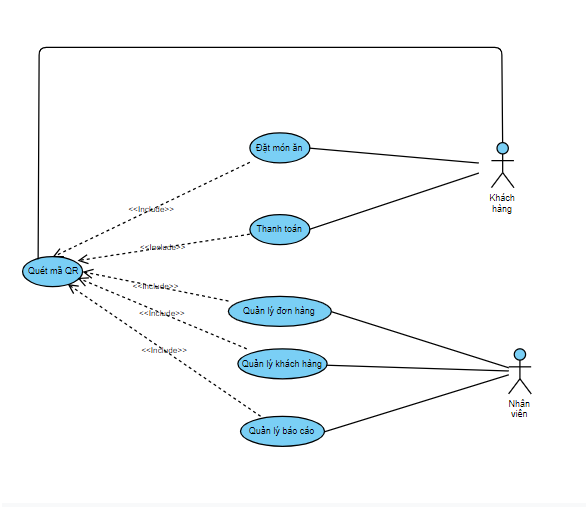
\includegraphics[width=1\textwidth]{Use-case-tong-quat.png}
    \caption{Use case tổng quan hệ thống.}
    \label{fig:Use-case-tong-quat}
\end{figure}

\section{Mô hình use case và đặc tả}

\subsection{Use case đăt món ăn}

\begin{figure}[H]
    \centering
    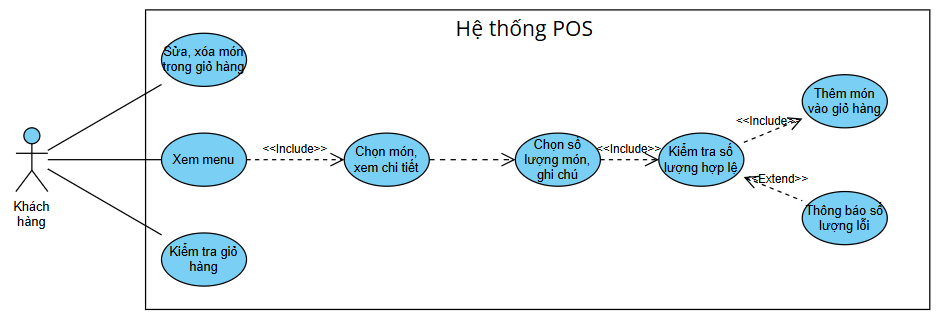
\includegraphics[width=1\linewidth]{Them_mon_vao_gio_hang.png}
    \caption{Use case đặt món ăn.}
    \label{fig:Them_mon_vao_gio_hang}
\end{figure}

\begin{table}[H]
    \small
    \centering
    \renewcommand{\arraystretch}{1.5} % Tăng khoảng cách giữa các dòng
    \setlength{\arrayrulewidth}{0.5mm} % Độ dày của đường kẻ
    \setlength{\tabcolsep}{5pt} % Khoảng cách giữa các cột
    \begin{tabularx}{\textwidth}{|l|X|}
        \hline
        \textbf{Use case}             & Đặt món ăn                                                                                                                               \\
        \hline
        \textbf{Tác nhân}             & Khách hàng                                                                                                                               \\
        \hline
        \textbf{Mô tả}                & Khách hàng sử dụng hệ thống POS để xem menu, chọn món, xem chi tiết từng món, chọn số lượng và thêm vào giỏ hàng.                        \\
        \hline
        \textbf{Điều kiện tiên quyết} & Đã truy cập hệ thống qua mã QR hoặc nền tảng web.                                                                                        \\
        \hline
        \textbf{Luồng sự kiện chính}  &
        1. Khách hàng xem menu. \newline
        2. Khách hàng chọn món để xem chi tiết. \newline
        3. Hệ thống hiển thị màn hình chi tiết món với thông tin đầy đủ. \newline
        4. Khách hàng chọn số lượng món muốn đặt và ghi chú món.  \newline
        5. Khách hàng thêm món vào giỏ hàng. \newline
        6. Hệ thống cập nhật giỏ hàng và hiển thị thông báo thêm món thành công. Khách hàng có thể tiếp tục chọn, sửa hoặc xóa món khỏi giỏ hàng.                                \\
        \hline
        \textbf{Luồng sự kiện phụ}    &
        $\rightarrow$ 4: Khách hàng nhập số lượng không hợp lệ hoặc món ăn đã hết hàng $\rightarrow$ Hệ thống sẽ thông báo cho khách hàng. \newline
        $\rightarrow$ 6: Nếu khách hàng muốn thay đổi số lượng món, hệ thống sẽ cập nhật giỏ hàng.                                                                               \\
        \hline
        \textbf{Kết quả}              & Món ăn đã được thêm vào giỏ hàng thành công. Khách hàng có thể tiếp tục chọn thêm món, kiểm tra giỏ hàng hoặc tiến hành thanh toán ngay. \\
        \hline
    \end{tabularx}

    \caption{Đặc tả use case đặt món ăn.}
    \label{fig:usecase-themmon}
\end{table}


\subsection{Use case thanh toán đơn hàng}
\begin{figure}[H]
    \centering
    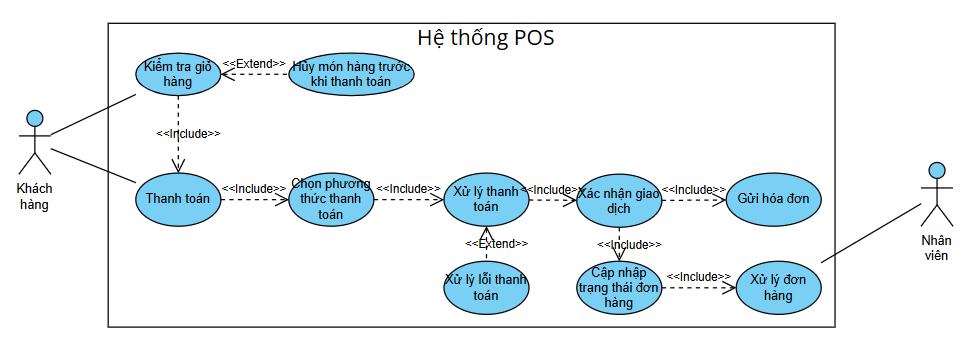
\includegraphics[width=1\linewidth]{Thanh_toan_don_hang.png}
    \caption{Use case thanh toán đơn hàng.}
    \label{fig:Thanh_toan_don_hang}
\end{figure}

\begin{table}[H]
    \small
    \centering
    \renewcommand{\arraystretch}{1.5} % Tăng khoảng cách giữa các dòng
    \setlength{\arrayrulewidth}{0.5mm} % Độ dày của đường kẻ
    \setlength{\tabcolsep}{5pt} % Khoảng cách giữa các cột
    \begin{tabularx}{\textwidth}{|l|X|}
        \hline
        \textbf{Use case}             & Thanh toán đơn hàng                                                                                               \\
        \hline
        \textbf{Tác nhân}             & Khách hàng, nhân viên nhà hàng                                                                                    \\
        \hline
        \textbf{Mô tả}                & Khách hàng kiểm tra giỏ hàng và tiến hành thanh toán. Hệ thống xử lý giao dịch và xác nhận thanh toán thành công. \\
        \hline
        \textbf{Điều kiện tiên quyết} &
        - Khách hàng đã có món trong giỏ hàng. \newline
        - Nhà hàng hỗ trợ phương thức thanh toán mà khách hàng sử dụng.                                                                                   \\
        \hline
        \textbf{Luồng sự kiện chính}  &
        1. Khách hàng kiểm tra giỏ hàng và thông tin đơn hàng. \newline
        2. Khách hàng chọn "Thanh toán". \newline
        3. Hệ thống hiển thị các phương thức thanh toán có sẵn (tiền mặt, thẻ, ví điện tử, QR code, v.v.). \newline
        4. Khách hàng chọn phương thức thanh toán.  \newline
        5. Hệ thống POS xử lý thanh toán. \newline
        6. Hệ thống xác nhận giao dịch thành công và cập nhật trạng thái đơn hàng thành "Đã thanh toán".\newline
        7. Hệ thống gửi hóa đơn điện tử hoặc in hóa đơn cho khách hàng.                                                                                   \\
        \hline
        \textbf{Luồng sự kiện phụ}    &
        $\rightarrow$ 5:  Nếu thanh toán thất bại, hệ thống hiển thị thông báo lỗi và cho phép khách hàng thử lại hoặc chọn phương thức khác. \newline
        $\rightarrow$ 2: Nếu khách hàng muốn hủy đơn trước khi thanh toán, hệ thống sẽ kiểm tra và cho phép hủy nếu đơn chưa được xác nhận. \newline
        $\rightarrow$ 6: Nếu khách hàng muốn thay đổi số lượng món, hệ thống sẽ cập nhật giỏ hàng.                                                        \\
        \hline
        \textbf{Kết quả}              &
        - Đơn hàng được thanh toán thành công, nhân viên nhà hàng tiếp nhận và xử lý đơn hàng. \newline
        - Hệ thống cập nhật trạng thái đơn hàng và gửi xác nhận thanh toán cho khách hàng.                                                                \\
        \hline
    \end{tabularx}

    \caption{Đặc tả use case thanh toán đơn hàng.}
    \label{fig:usecase-thanh-toan}
\end{table}


\subsection{Use case xử lý đơn hàng}
\begin{figure}[H]
    \centering
    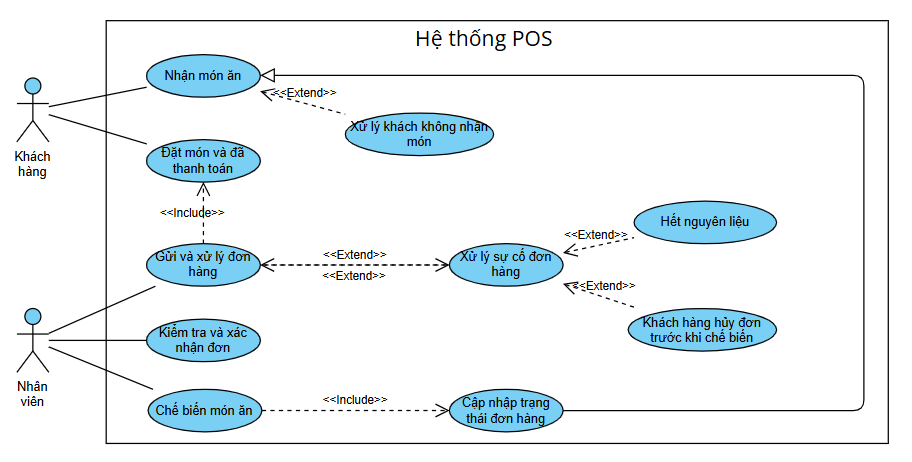
\includegraphics[width=1\linewidth]{Xu_ly_don_hang.png}
    \caption{Use case xử lý đơn hàng.}
    \label{fig:Xu_ly_don_hang}
\end{figure}

\begin{table}[H]
    \small
    \centering
    \renewcommand{\arraystretch}{1.5} % Tăng khoảng cách giữa các dòng
    \setlength{\arrayrulewidth}{0.5mm} % Độ dày của đường kẻ
    \setlength{\tabcolsep}{5pt} % Khoảng cách giữa các cột
    \begin{tabularx}{\textwidth}{|l|X|}
        \hline
        \textbf{Use case}             & Xử lý đơn hàng                                                                     \\
        \hline
        \textbf{Tác nhân}             & Khách hàng, nhân viên nhà hàng                                                     \\
        \hline
        \textbf{Mô tả}                & Nhân viên tiếp nhận đơn hàng từ hệ thống POS. Sau đó xử lý đơn hàng.               \\
        \hline
        \textbf{Điều kiện tiên quyết} &
        - Khách hàng truy cập vào hệ thống POS và đã thanh toán. \newline
        - Nhà hàng có sẵn món ăn trong thực đơn.                                                                           \\
        \hline
        \textbf{Luồng sự kiện chính}  &
        1. Hệ thống POS gửi đơn hàng của khách hàng đến nhà hàng. \newline
        2. Nhân viên nhà hàng kiểm tra đơn hàng. \newline
        3. Nhân viên nhà hàng xác nhận đơn hàng và bắt đầu chế biến món ăn. \newline
        4. Hệ thống POS cập nhật trạng thái đơn hàng thành "Đang chuẩn bị".  \newline
        5. Nhân viên nhà hàng hoàn thành món ăn và cập nhật trạng thái đơn hàng thành "Hoàn thành". \newline
        6. Hệ thống POS gửi thông báo cho khách hàng rằng món ăn đã sẵn sàng để phục vụ hoặc giao đi.\newline
        7. Khách hàng nhận món tại bàn hoặc nhận hàng tại quầy nếu mang đi.                                                \\
        \hline
        \textbf{Luồng sự kiện phụ}    &
        $\rightarrow$ 3.1: Nếu nhà hàng không thể chế biến món ăn do hết nguyên liệu $\rightarrow$ Hệ thống POS thông báo cho khách hàng. \newline
        $\rightarrow$ 3.2: Nếu khách hàng muốn hủy đơn trước khi chế biến $\rightarrow$ Hệ thống POS xử lý yêu cầu hủy đơn nếu chưa vào giai đoạn chế biến. \newline
        $\rightarrow$ 7: Nếu khách hàng không nhận món sau thời gian quy định → Nhà hàng có thể xử lý tùy theo chính sách. \\
        \hline
        \textbf{Kết quả}              &
        - Món ăn được chế biến và giao cho khách hàng. \newline
        - Trạng thái đơn hàng được cập nhật trong hệ thống.                                                                \\
        \hline
    \end{tabularx}

    \caption{Đặc tả use case xử lý đơn hàng.}
    \label{tab:usecase-don-hang}
\end{table}


\section{Mô hình hóa hệ thống}
\subsection{Sơ đồ hoạt động (Activity diagram)}
\begin{figure}[H]
    \centering
    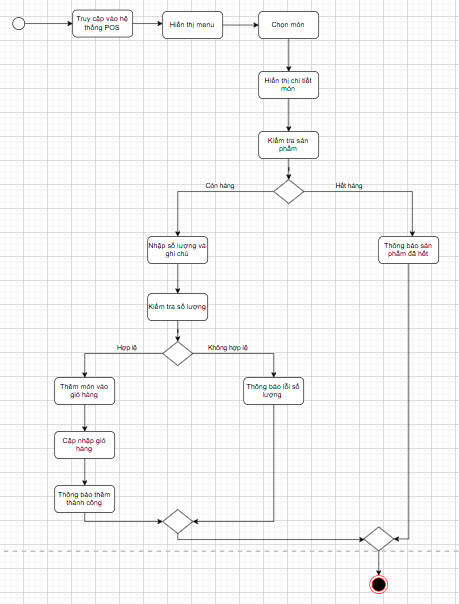
\includegraphics[width=1\linewidth]{activity-them-mon-an.jpg}
    \caption{Sơ đồ đồ hoạt động đặt món ăn.}
    \label{fig:activity-them-mon-an}
\end{figure}

\subsection{Sơ đồ trình tự (Sequence diagram)}
\begin{figure}[H]
    \centering
    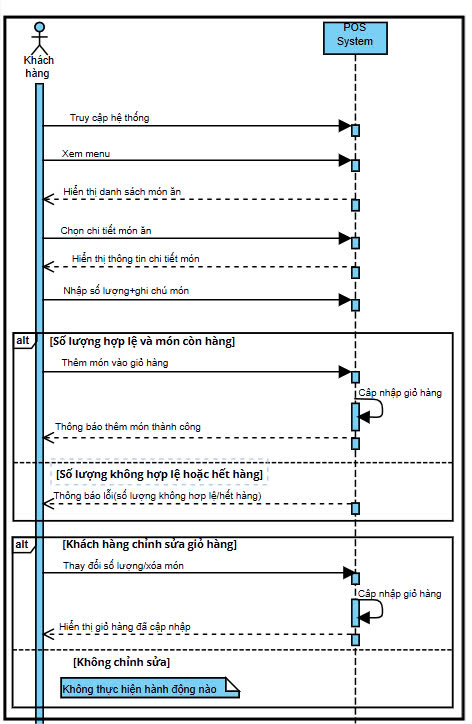
\includegraphics[width=1\linewidth]{sequence-them-mon-an.jpg}
    \caption{Sơ đồ trình tự đặt món ăn.}
    \label{fig:sequence-them-mon-an}
\end{figure}

\begin{figure}[H]
    \centering
    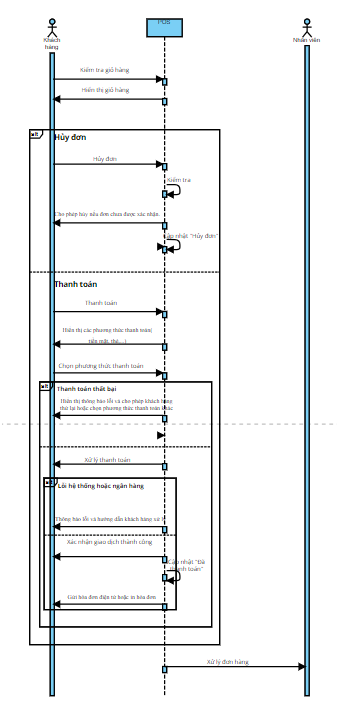
\includegraphics[width=0.78\linewidth]{sequence-thanh-toan.png}
    \caption{Sơ đồ trình tự thanh toán.}
    \label{fig:sequence-thanh-toan}
\end{figure}

\begin{figure}[H]
    \centering
    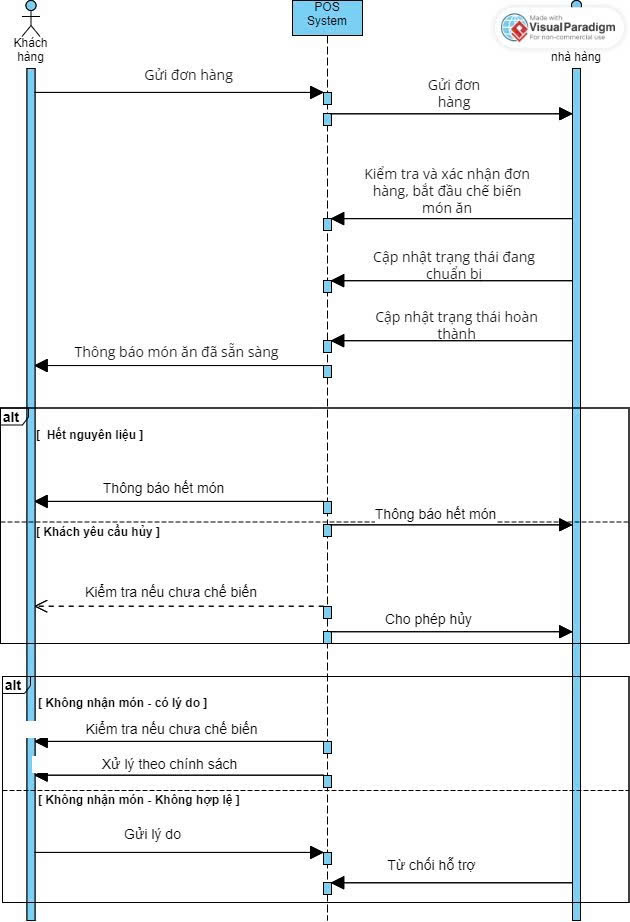
\includegraphics[width=1\linewidth]{sequence-don-hang.jpg}
    \caption{Sơ đồ trình tự xử lý đơn hàng}
    \label{fig:sequence-don-hang}
\end{figure}

\subsection{Sơ đồ lớp (Class Diagram)}
\begin{figure}[H]
    \centering
    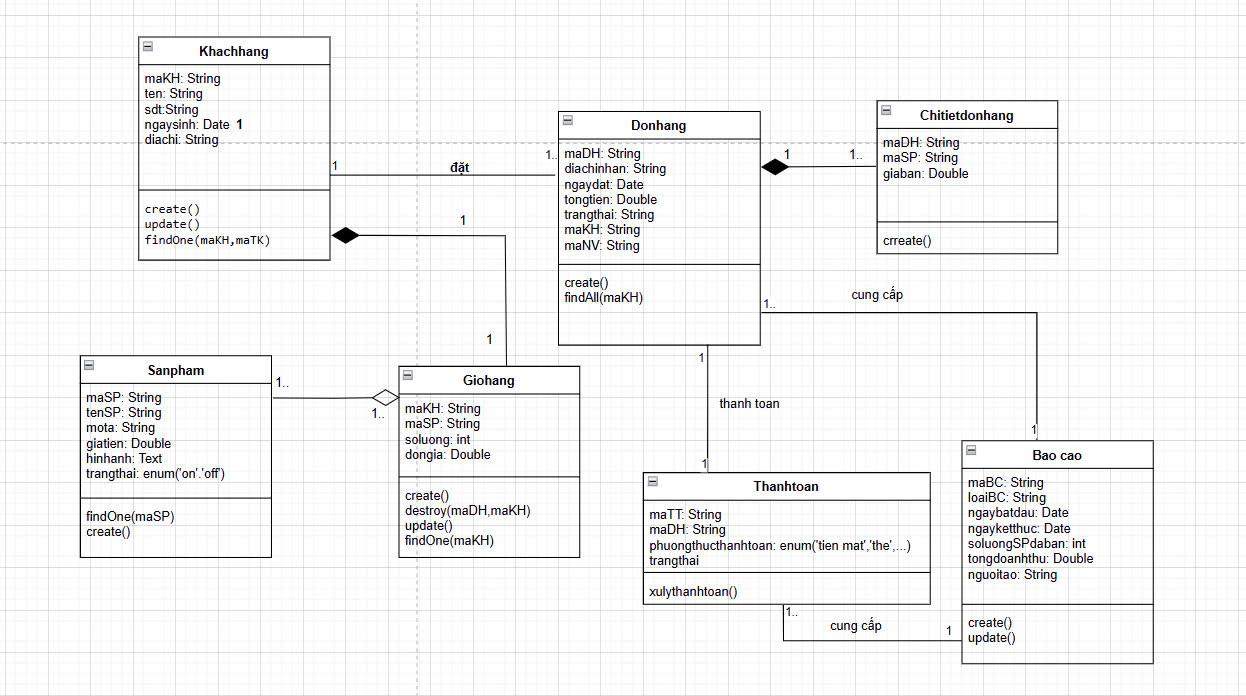
\includegraphics[width=1\linewidth]{so-so-lop-he-thong.jpg}
    \caption{Sơ đồ lớp hệ thống bán hàng POS.}
    \label{fig:so-so-lop-he-thong}
\end{figure}
\section{Thiết kế kiến trúc}
\subsection{Tổng quan kiên trúc hệ thống}
\quad Hệ thống POS (Point of Sale) được thiết kế để quản lý quy trình bán hàng, bao gồm việc theo dõi sản phẩm, quản lý đơn hàng, người dùng và xử lý thanh toán. Hệ thống được xây dựng bằng Next.js, sử dụng MySQL (trên XAMPP) làm cơ sở dữ liệu và Prisma ORM để tương tác với CSDL.

\vspace{0.8em}

\quad Kiến trúc hệ thống được xây dựng theo mô hình Monolithic kết hợp với phân lớp (Layered Architecture), nơi giao diện người dùng, logic nghiệp vụ và truy cập dữ liệu được tổ chức rõ ràng, giúp dễ mở rộng và bảo trì.

\subsection{Kiến trúc hệ thống}
\begin{enumerate}[label=\textbf{\alph*.}]
    \item \textbf{Kiến trúc tổng thể} \\
          \sloppy Hệ thống sử dụng kiến trúc Monolithic App trong môi trường Next.js, trong đó toàn bộ frontend, backend (API) và data access được triển khai trong một ứng dụng duy nhất. Kiến trúc này phù hợp cho các ứng dụng nhỏ và vừa, dễ triển khai và giảm độ phức tạp ban đầu.
    \item \textbf{Các lớp trong kiến trúc}
          \begin{table}[H]
              \small
              \centering
              \renewcommand{\arraystretch}{1.5} % Tăng khoảng cách giữa các dòng
                \setlength{\arrayrulewidth}{0.5mm} % Độ dày của đường kẻ
                 \setlength{\tabcolsep}{5pt} % Khoảng cách giữa các cột
              \begin{tabularx}{\textwidth}{|>{\raggedright\arraybackslash}p{5cm}|X|}
                  \hline
                  \textbf{Lớp}                                       & \textbf{Mô tả}                                                                                                                                    \\
                  \hline
                  \textbf{Giao diện người dùng (Presentation Layer)} & Xây dựng bằng các React Component trong \textbf{components}, quản lý layout và routing trong \textbf{app/} hoặc \textbf{pages/}.                  \\
                  \hline
                  \textbf{Logic nghiệp vụ (Business Logic Layer)}    & Chứa các hàm logic xử lý tính toán, xác thực, định dạng dữ liệu, ... được tổ chức trong thư mục \textbf{lib/} hoặc đặt trực tiếp trong API route. \\
                  \hline
                  \textbf{Truy cập dữ liệu (Data Access Layer)}      & Sử dụng Prisma ORM để tương tác với MySQL, định nghĩa mô hình trong \textbf{prisma/schema.prisma}.                                                \\
                  \hline
              \end{tabularx}
          \end{table}
    \item  \textbf{Các thành phần chính}
          \begin{itemize}
              \item Frontend (UI):
                    \begin{itemize}
                        \item Next.js + React: Hiển thị giao diện người dùng.
                        \item Components: Các phần tử UI trong components/.
                        \item Tailwind CSS/ CSS Modules: Thiết kế giao diện hiện đại, tiện tùy biến.
                    \end{itemize}
              \item Backend (API):
                    \begin{itemize}
                        \item API Routes/ Server Actions: Các route xử lý backend được viết trong pages/api/ hoặc app/api/ (tùy App Router).
                        \item Lib hàm xử lý logic: Dùng để chia nhỏ các nghiệp vụ phức tạp.
                    \end{itemize}
              \item ORM và CSDL:
                    \begin{itemize}
                        \item Prisma ORM: Cầu nối giữa backend và CSDL, giúp viết truy vấn dễ hiểu, bảo mật và dễ bảo trì.
                        \item MySQL (XAMPP): Lưu trữ dữ liệu người dùng, sản phẩm, loại sản phẩm, ...
                    \end{itemize}
          \end{itemize}
    \item \textbf{Luồng dữ liệu tổng quát}
          \begin{enumerate}[label=B\arabic*.]
              \item Người dùng mở ứng dụng thông qua trình duyệt.
              \item Người dùng mở ứng dụng thông qua trình duyệt.
              \item API route xử lý nghiệp vụ, gọi hàm trong lib/ xác thực thông tin nếu cần.
              \item Prisma ORM truy vấn hoặc cập nhật dữ liệu trong MySQL.
              \item Kết quả trả về API, sau đó cập nhật lại giao diện người dùng.
          \end{enumerate}
\end{enumerate}
%\subsection{Sơ đồ triển khai (Deployment Diagram)}

\section{Triển khai - Sprint 1}
\subsection{Triển khai MVP cho màn hình Menu}
\begin{itemize}
    \item Mục tiêu: Xây dựng phiên bản cơ bản đầu tiên của màn hình Menu.
    \item Công việc thực hiện:
          \begin{itemize}
              \item Thiết kế giao diện cơ bản (dùng Figma).
              \item Xây dựng màn hình giao diện với các mục:
                    \begin{itemize}
                        \item Giao diện đăng nhập và đăng ký
                        \item Giao diện menu
                        \item Giao diện chi tiết món ăn
                        \item Giao diện thanh toán
                    \end{itemize}
              \item Giao diện thân thiện, dễ sử dụng
          \end{itemize}
\end{itemize}
\subsection{Thiết lập dự án}
\begin{itemize}
    \item Mục tiêu: Khởi tạo môi trường làm việc ban đầu để phát triển phần~mềm.
    \item Công việc cụ thể:
          \begin{itemize}
              \item Chọn công nghệ và ngôn ngữ lập trình phù hợp (NextJS).
              \item Khởi tạo repository trên GitHub/GitLab.
          \end{itemize}
    \item Cấu hình môi trường làm việc:
          \begin{itemize}
              \item Cài đặt công cụ lập trình (VS Code)
              \item Tạo các project rỗng
              \item Thiết lập quản lý phiên bản với Git (git init, .gitignore).
              \item Cài đặt các thư viện/chức năng cơ bản cần thiết
          \end{itemize}
\end{itemize}
\subsection{Tổ chức thư mục và tài liệu}
\begin{forest}
    for tree={
    font=\ttfamily,
    grow'=0,
    child anchor=west,
    parent anchor=south,
    anchor=west,
    calign=first,
    edge path={
            \noexpand\path [draw, \forestoption{edge}]
            (!u.south west) ++(5pt,0) -- +(5pt,0) |- (.child anchor)\forestoption{edge label};
        },
    before typesetting nodes={
            if n=1
                {insert before={[,phantom]}}{},
        },
    fit=band,
    before computing xy={l=10pt},
    scale=0.8,
    }
    [src/
    [components/
    [Cart.tsx]
    [Login.tsx]
    [Menu.tsx]
    [Pay.tsx]
    [ProductDetail.tsx]
    [Register.tsx]
    ]
    [pages/
    [api/
    [auth.ts]
    [hello.ts]
    ]
    [\_app.tsx]
    [\_document.tsx]
    [index.tsx]
    [menu.tsx]
    [pay.tsx]
    [register.tsx]
    ]
    [styles/
    [Login.module.css]
    [Menu.module.css]
    [Payment.css]
    [ProductDetail.module.css]
    [Register.module.css]
    [globals.css]]
    [utils/
    [auth.ts]]
    [types/
    [index.ts]]
    ]
\end{forest}
\section{Kiểm thử}
\subsection{Test design}
\begin{itemize}
    \item Chọn 2 module chính để kiểm thử là Đăng nhập và Đăng ký.
\end{itemize}
\begin{center}
    \renewcommand{\arraystretch}{1.5} % Tăng khoảng cách giữa các dòng
    \setlength{\arrayrulewidth}{0.5mm} % Độ dày của đường kẻ
    \setlength{\tabcolsep}{5pt} % Khoảng cách giữa các cột
    \begin{longtable}{|>{\centering\arraybackslash}m{4cm}|
        >{\centering\arraybackslash}m{4cm}|
        >{\raggedright\arraybackslash}m{7.5cm}|}
        \hline
        \textbf{Các module và chức năng} & \textbf{TR\#} & \textbf{Description} \\
        \hline
        \multirow{6}{=}{\centering Đăng nhập} 
        & T1 & Email đăng nhập không để trống. \\
        \cline{2-3}
        & T2 & Mật khẩu không được để trống. \\
        \cline{2-3}
        & T3 & Nếu Email và mật khẩu đúng thì đăng nhập vào hệ thống. \\
        \cline{2-3}
        & T4 & Nếu Email đúng – mật khẩu sai thì thông báo lỗi. \\
        \cline{2-3}
        & T5 & Nếu Email sai thì thông báo tài~khoản không tồn tại. \\
        \cline{2-3}
        & T6 & Nếu người dùng nhấn biểu tượng hiển password bên phải ô đăng nhập thì sẽ hiển password. \\
        \hline
        \multirow{5}{=}{\centering Đăng ký ngay} 
        & T7 & Email đăng nhập không để trống. \\
        \cline{2-3}
        & T8 & Mật khẩu không được để trống. \\
        \cline{2-3} 
        & T9 & Xác nhận mật khẩu không được để trống. \\
        \cline{2-3} 
        & T10 & Nếu Email và mật khẩu đúng thì đăng nhập vào hệ thống. \\
        \cline{2-3}
        & T11 & Nếu Email đúng – mật khẩu và xác nhận mật khẩu không trùng khớp thì thông báo lỗi. \\
        \hline
    \end{longtable}
\end{center}
\newpage
\subsection{Test case}
    \renewcommand{\arraystretch}{1.5} % Tăng khoảng cách giữa các dòng
    \setlength{\arrayrulewidth}{0.5mm} % Độ dày của đường kẻ
    \setlength{\tabcolsep}{5pt} % Khoảng cách giữa các cột
    \begin{longtable}{|
    >{\centering\arraybackslash}p{1cm}|
    >{\centering\arraybackslash}p{2cm}|
    >{\raggedright\arraybackslash}p{2.5cm}|
    >{\centering\arraybackslash}p{4cm}|
    >{\centering\arraybackslash}p{2cm}|
    >{\centering\arraybackslash}p{1.5cm}|
    >{\centering\arraybackslash}p{1.3cm}|}
        \hline
        \rowcolor{pink!30} 
        \textbf{Test case ID} & \textbf{Test case} & \centering\textbf{Test steps} & \textbf{Test data} & \textbf{Expected result} & \textbf{Actual result} & \textbf{Pass/ Failed} \\
        \hline
        T1 & Kiểm tra phản hồi của chương trình nếu để trống Email & 
        1) Vào trang đăng nhập \newline
        2) Nhập dữ liệu vào ô mật khẩu \newline
        3) Nhấn nút đăng nhập & 
        Mk:123456 & 
        Hiển thị thông báo Email không để trống & 
        Hiển thị thông báo Email không để trống & 
        Pass \\
        \hline
        T2 & Kiểm tra phản hồi của chương trình nếu mật khẩu để trống & 
        1) Vào trang đăng nhập \newline
        2) Nhập dữ liệu vào ô Email \newline
        3) Ấn nút đăng nhập & 
        Tk:abc@gmail.com & 
        Hiển thị thông báo mật khẩu không được để trống & 
        Hiển thị thông báo lỗi mật khẩu & 
        Pass \\
        \hline
        T3 & Kiểm tra phản hồi của chương trình nếu Email và mật khẩu đúng thì đăng nhập vào ứng dụng & 
        1) Vào trang đăng nhập \newline
        2) Nhập Email và mật khẩu \newline
        3) Ấn nút đăng nhập & 
        Tk:abc@gmail.com \newline
        Mk:123456 & 
        Hiển thị thông báo đăng nhập thành công & 
        Hiển thị thông báo đăng nhập thành công & 
        Pass \\
        \hline
        T4 & Kiểm tra phản hồi của chương trình nếu Email đúng – mật khẩu sai & 
        1) Vào trang đăng nhập \newline
        2) Nhập Email và mật khẩu \newline
        3) Ấn nút đăng nhập & 
        Tk:abc@gmail.com \newline
        Mk:123 \newline
        Mk đúng:123456 & 
        Hiển thị thông báo mật khẩu sai & 
        Hiển thị thông báo mật khẩu sai & 
        Pass \\
        \hline
        T5 & Kiểm tra phản hồi của chương trình nếu Email thì thông báo tài khoản không tồn tại & 
        1) Vào trang đăng nhập \newline
        2) Nhập Email và mật khẩu \newline
        3) Ấn nút đăng nhập & 
        Tk:abc \newline & 
        Hiển thị thông báo mật khẩu sai & 
        Hiển thị thông báo mật khẩu sai & 
        Pass \\
        \hline
        T6 & Kiểm tra phản hồi của chương trình nếu nhấn biểu tượng hiện password & 
        1) Vào trang đăng nhập \newline
        2) Nhập dữ liệu vào ô mật khẩu \newline
        3) Nhấn nút hiện password & 
        Mk đúng:123456 & 
        Hiện password vừa nhập & 
        Hiện password vừa nhập & 
        Pass \\
        \hline
        T7 & Kiểm tra phản hồi của chương trình nếu để trống Email & 
        1) Vào trang đăng ký \newline
        2) Nhập dữ liệu vào ô mật khẩu \newline
        3) Nhấn nút đăng ký & 
        Mk:123456 & 
        Hiện thị thông báo Email không để trống & 
        Hiển thị thông báo Email không để trống & 
        Pass \\
        \hline
        T8 & Kiểm tra phản hồi của chương trình nếu mật khẩu để trống & 
        1) Vào trang đăng ký \newline
        2) Nhập dữ liệu vào ô mật khẩu \newline
        3) Nhấn nút đăng ký & 
        Tk:abc@gmail.com \newline
        Xnmk: 123456 & 
        Hiển thị thông báo mật khẩu không để trống & 
        Hiện thị thông báo lỗi mật khẩu & 
        Pass \\
        \hline
        T9 & Kiểm tra phản hồi của chương trình nếu xác nhận mật khẩu để trống & 
        1) Vào trang đăng ký \newline
        2) Nhập dữ liệu vào ô mật khẩu \newline
        3) Nhấn nút đăng ký & 
        Tk:abc@gmail.com \newline
        Mk:123456 & 
        Hiển thị thông báo xác nhận mật khẩu không để trống & 
        Hiện thị thông báo lỗi xác nhận mật khẩu & 
        Pass \\
        \hline
        T10 & Kiểm tra phản hồi của chương trình nếu Email và mật khẩu đúng thì đăng nhập vào hệ thống & 
        1) Vào trang đăng ký \newline
        2) Nhập Email, mật khẩu và xác nhận mật khẩu \newline
        3) Ấn nút đăng ký & 
        Tk:abc@gmail.com \newline
        Mk:123456 \newline
        Xnmk:123456 & 
        Hiển thị thông báo đăng ký thành công & 
        Hiển thị thông báo đăng ký thành công & 
        Pass \\
        \hline
        T11 & Kiểm tra phản hồi của chương trình nếu mật khẩu và xác nhận mật khẩu không trùng khớp & 
        1) Vào trang đăng ký \newline
        2) Nhập dữ liệu vào ô mật khẩu \newline
        3) Nhấn nút đăng ký & 
        Tk:abc@gmail.com \newline
        Mk đúng:123456 \newline
        Xnmk sai:123  & 
        Hiện thị thông báo mật khẩu xác nhận không khớp  & 
        Hiện thị thông báo mật khẩu xác nhận không khớp  & 
        Pass \\
        \hline
    \end{longtable}
\section{Triển khai - Sprint 2}
\subsection{Giao diện}
\subsubsection{Giao diện đăng nhập}
\begin{figure}[H]
    \centering
    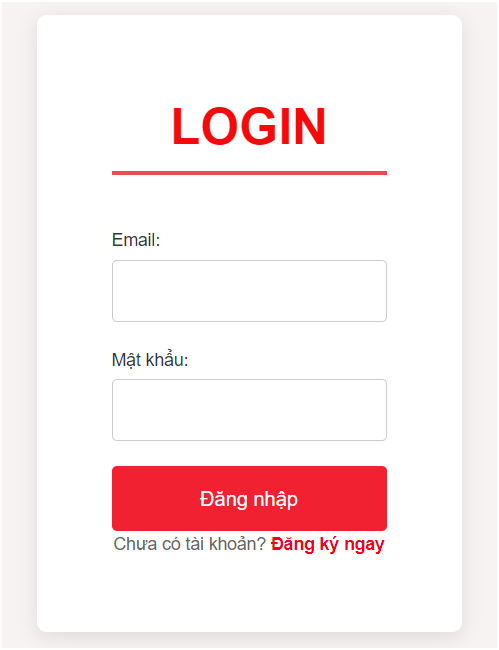
\includegraphics[width=0.5\linewidth]{login.png}
    \caption{Giao diện đăng nhập của khách hàng.}
    \label{fig:login}
\end{figure}
\subsubsection{Giao diện đăng ký}
\begin{figure}[H]
    \centering
    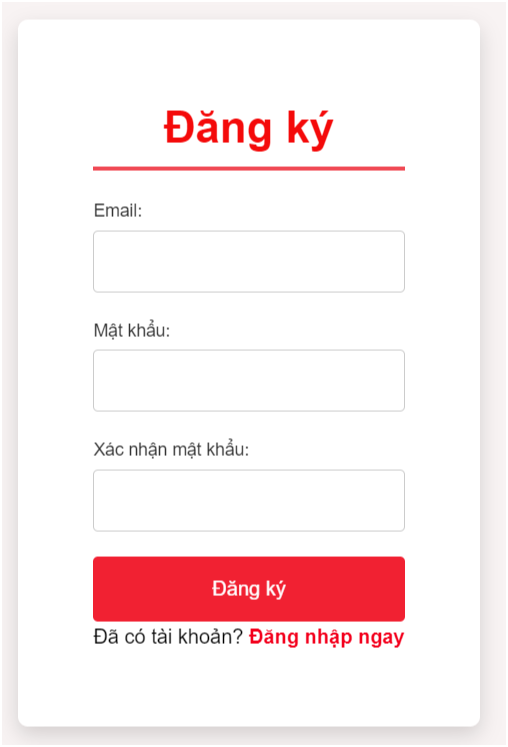
\includegraphics[width=0.5\linewidth]{dangky.png}
    \caption{Giao diện đăng ký của khách hàng.}
    \label{fig:dangky}
\end{figure}
\subsubsection{Giao diện menu}
\begin{figure}[H]
    \centering
    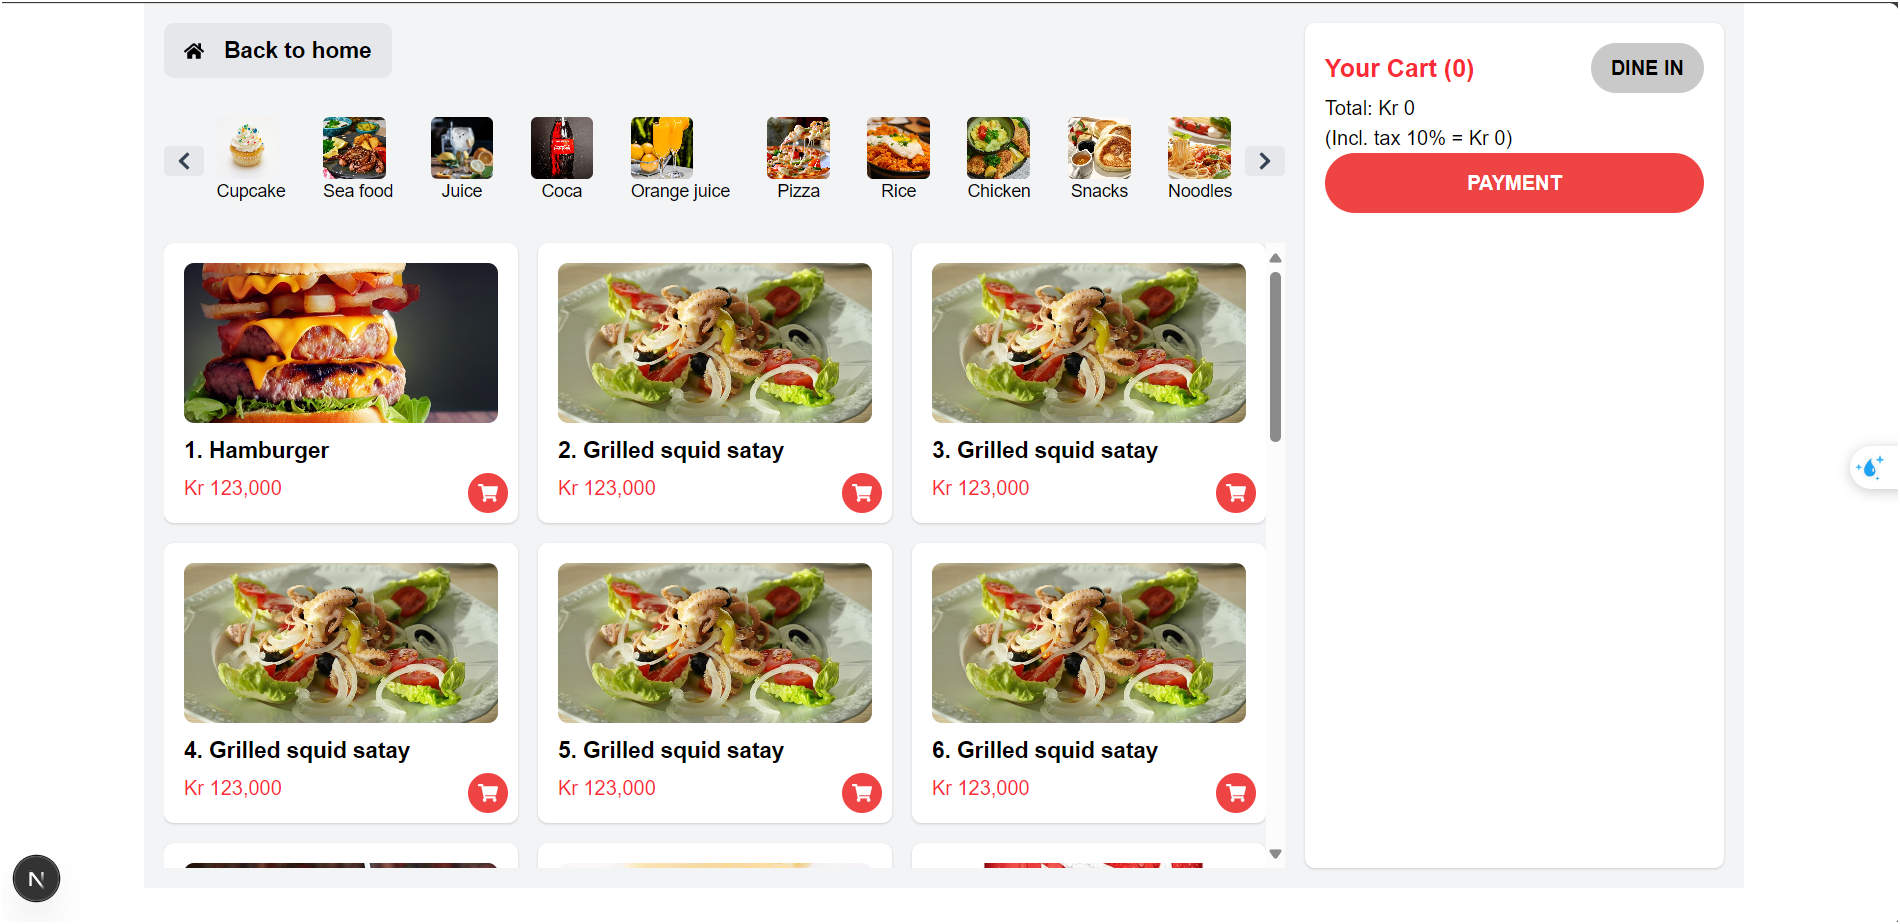
\includegraphics[width=0.8\linewidth]{menu.png}
    \caption{Giao diện menu của khách hàng.}
    \label{fig:menu}
\end{figure}
\subsubsection{Giao diện chi tiết món ăn}
\begin{figure}[H]
    \centering
    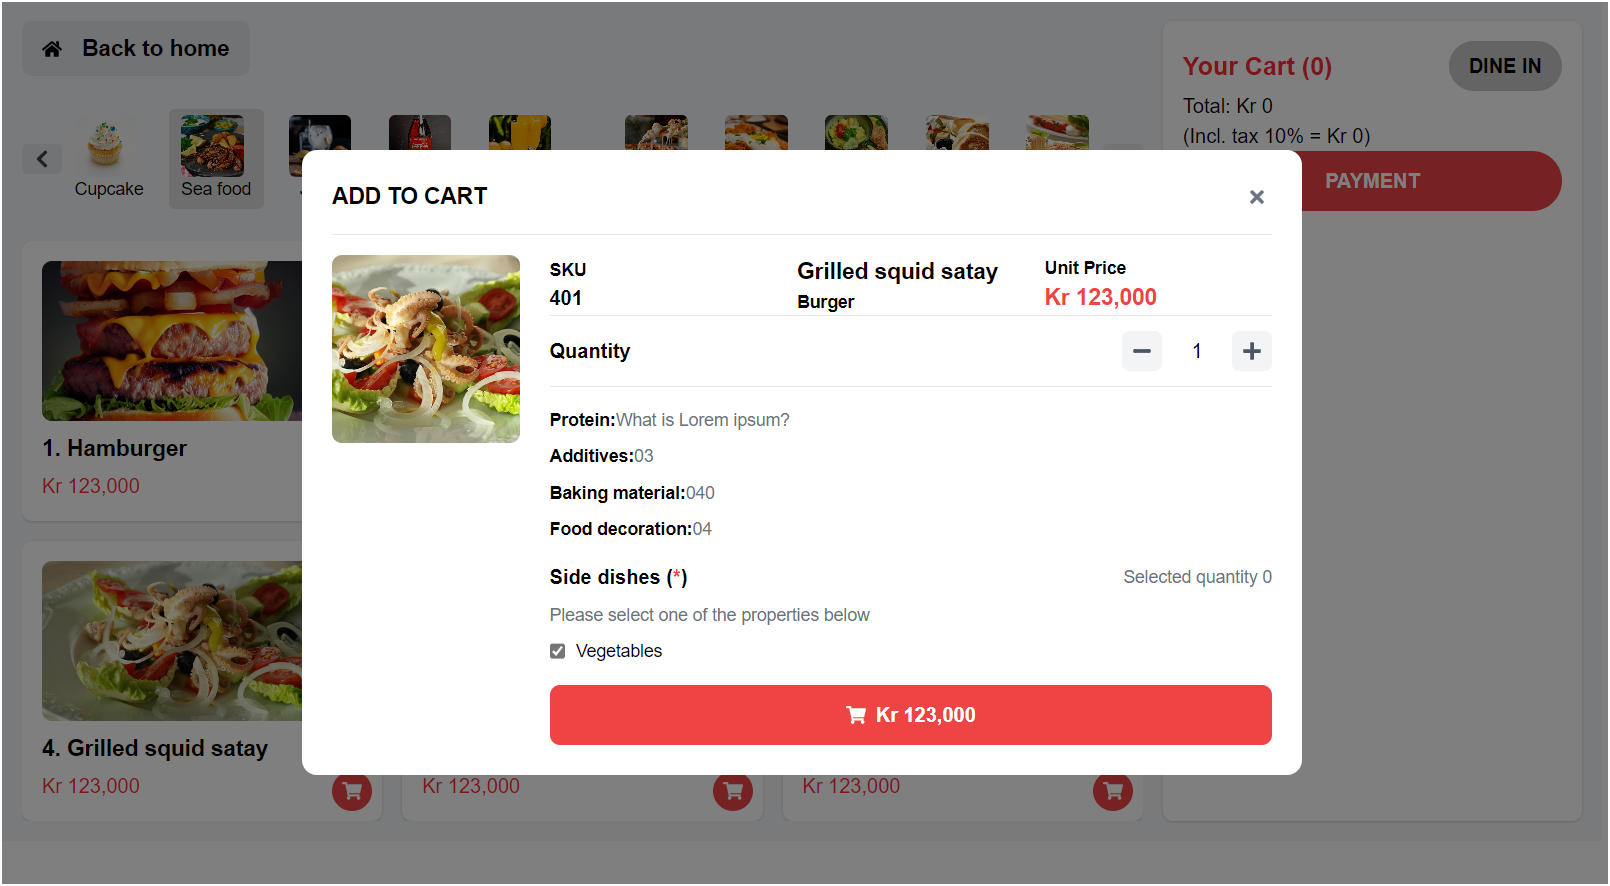
\includegraphics[width=0.8\linewidth]{chi-tiet-san-pham.png}
    \caption{Giao diện chi tiết món ăn của khách hàng.}
    \label{fig:chi-tiet-san-pham}
\end{figure}
\subsubsection{Giao diện thanh toán}
\begin{figure}[H]
    \centering
    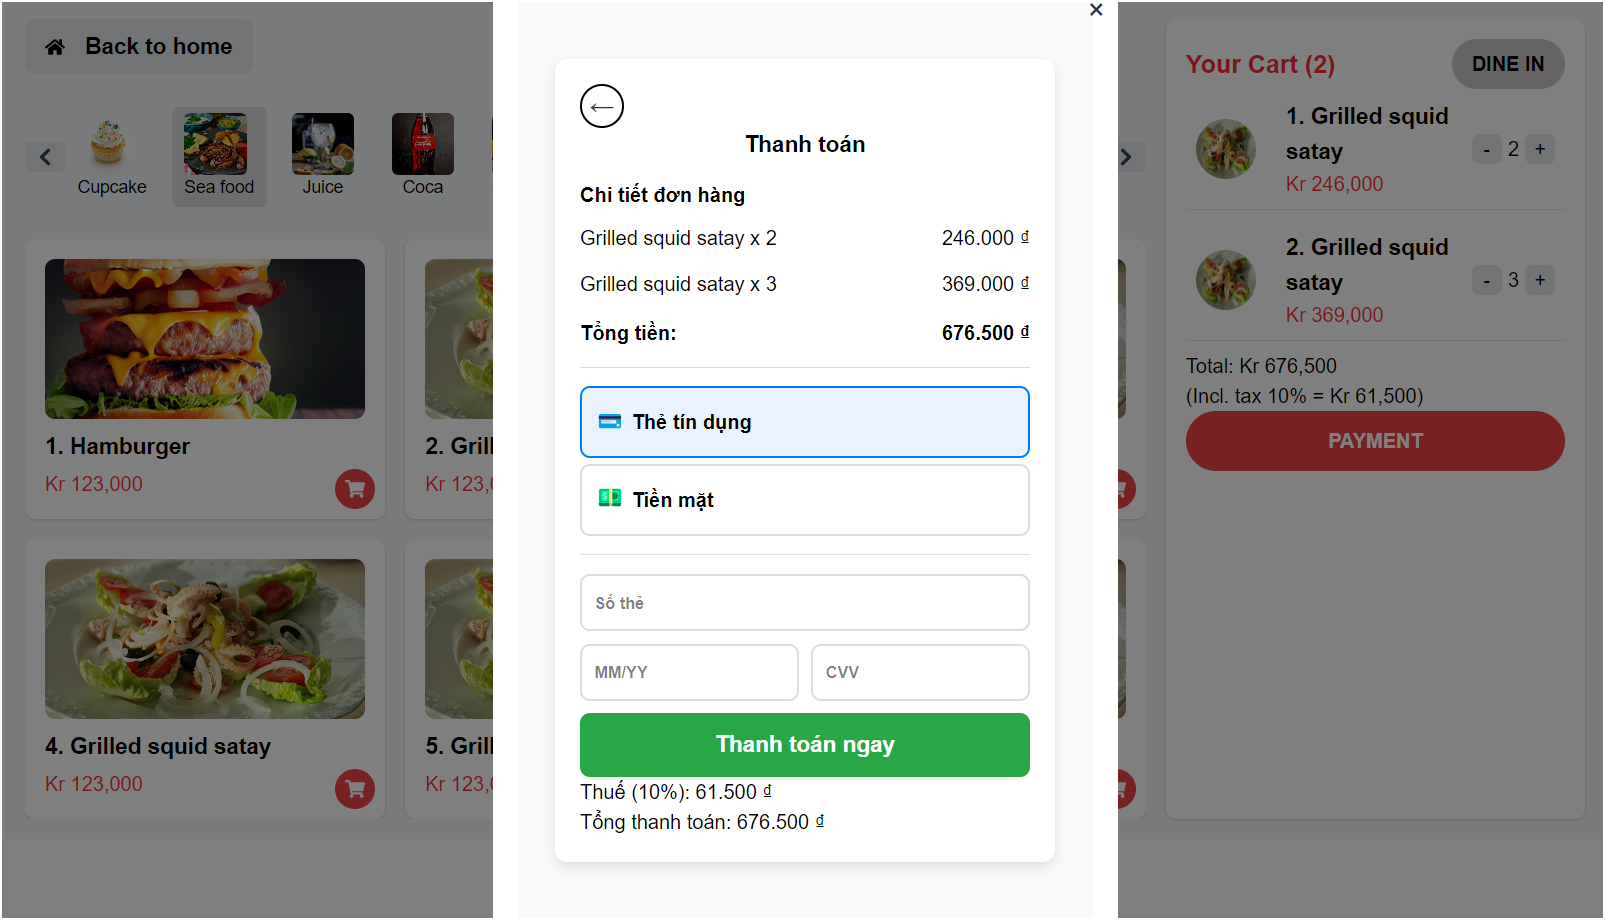
\includegraphics[width=0.8\linewidth]{thanh-toan.png}
    \caption{Giao diện thanh toán của khách hàng.}
    \label{fig:thanh-toan}
\end{figure}
\subsection{Hướng dẫn sử dụng hệ thống}
\subsubsection{Đăng ký tài khoản}
\begin{tabularx}{\textwidth}{|>{\raggedright\arraybackslash}p{5cm}|X|}
    \hline
    \textbf{Tên mục hướng dẫn}  & Đăng ký tài khoản                                                                                                 \\
    \hline
    \textbf{Các bước thực hiện} &
    \begin{minipage}[t]{\linewidth}
        \begin{enumerate}
            \item Ở trang đăng nhập người dùng nhấn chọn nút "Đăng ký ngay".
            \item Ở trang đăng ký người dùng nhập các thông tin được hiển thị gồm email, mật khẩu và xác nhận mật khẩu.
            \item Sau đó nhấn nút "Đăng ký".
            \item Hệ thống thông báo "Đăng ký thành công!" nhấn "OK".
        \end{enumerate}
    \end{minipage}
    \\
    \hline
    \textbf{Lưu ý}              & Nếu người dùng nhập thông tin không hợp lệ, hệ thống sẽ hiển thị thông báo lỗi và yêu cầu nhập lại.               \\
    \hline
    \textbf{Kết quả}            & Người dùng đã đăng ký thành công, hệ thống sẽ tự động chuyển về trang đăng nhập và có thể đăng nhập vào hệ thống. \\
    \hline
\end{tabularx}

\subsubsection{Đăng nhập}
\begin{tabularx}{\textwidth}{|>{\raggedright\arraybackslash}p{5cm}|X|}
    \hline
    \textbf{Tên mục hướng dẫn}  & Đăng nhập                                                                                                          \\
    \hline
    \textbf{Các bước thực hiện} &
    \begin{minipage}[t]{\linewidth}
        \begin{enumerate}
            \item Người dùng truy cập trang đăng nhập và nhập email và mật khẩu của tài khoản đăng đăng ký thành công trước đó.
            \item Sau đó bấm nút "Đăng nhập".
        \end{enumerate}
    \end{minipage}
    \\
    \hline
    \textbf{Lưu ý}              & Nếu chưa có tài khoản thì chọn "Đăng ký ngay" để đăng ký. Nếu mật khẩu sai, hệ thống sẽ yêu cầu nhập lại mật khẩu. \\
    \hline
    \textbf{Kết quả}            & Người dùng chuyển về trang chính của website.                                                                      \\
    \hline
\end{tabularx}
\subsubsection{Xem chi tiết món ăn}

\begin{tabularx}{\textwidth}{|>{\raggedright\arraybackslash}p{5cm}|X|}
    \hline
    \textbf{Tên mục hướng dẫn}  & Xem chi tiế món ăn                                                                                             \\
    \hline
    \textbf{Các bước thực hiện} &
    \begin{minipage}[t]{\linewidth}
        \begin{enumerate}
            \item Người dùng nhấn vào nút giỏ hàng trên món ăn bất kỳ trong menu để xem chi tiết.
            \item Hệ thống hiển thị thông tin chi tiết, người dùng xem và lựa chọn các mục cần thiết.
        \end{enumerate}
    \end{minipage}
    \\
    \hline
    \textbf{Lưu ý}              & Nếu món ăn chưa có thông tin chi tiết, hệ thống sẽ hiển thị thông báo "Thông tin chưa có sẵn".                 \\
    \hline
    \textbf{Kết quả}            & Người dùng được hiển thị thông tin chi tiết món ăn, bao gồm tên, mô tả, giá, nguyên liệu, món kèm và hình ảnh. \\
    \hline
\end{tabularx}

\subsubsection{Chọn món và thêm vào giỏ hàng}

\begin{tabularx}{\textwidth}{|>{\raggedright\arraybackslash}p{5cm}|X|}
    \hline
    \textbf{Tên mục hướng dẫn}  & Chọn món và thêm vào giỏ hàng                                                                                                     \\
    \hline
    \textbf{Các bước thực hiện} &
    \begin{minipage}[t]{\linewidth}

        \begin{enumerate}
            \item Người dùng duyệt danh mục món ăn.
            \item Xem chi tiết, tùy chỉnh số lượng.
            \item Chọn món và bấm nút "Thêm vào giỏ hàng".
        \end{enumerate}
    \end{minipage}
    \\
    \hline
    \textbf{Lưu ý}              & Nếu món ăn đã có trong giỏ hàng, hệ thống sẽ hiển thị món ăn trong giỏ hàng, người dùng có thể tùy chỉnh số lượng trong giỏ hàng. \\
    \hline
    \textbf{Kết quả}            & Món ăn được thêm vào giỏ hàng thành công, người dùng có thể thanh toán.                                                           \\
    \hline
\end{tabularx}

\subsubsection{Thanh toán}
\begin{tabularx}{\textwidth}{|>{\raggedright\arraybackslash}p{5cm}|X|}
    \hline
    \textbf{Tên mục hướng dẫn}  & Thanh toán                                                                                           \\
    \hline
    \textbf{Các bước thực hiện} &
    \begin{minipage}[t]{\linewidth}
        \begin{enumerate}
            \item Người dùng bấm nút "Payment".
            \item Hệ thống hiển thị chi tiết thanh toán.
            \item Người dùng xem, kiểm tra và lựa chọn phương thức thanh toán.
            \item Nhấn nút vào "Thanh toán ngay".
        \end{enumerate}
    \end{minipage}
    \\
    \hline
    \textbf{Lưu ý}              & Nếu chọn phương thức thanh toán bằng thẻ, người dùng cần nhập số thẻ và các thông tin chi tiết khác. \\
    \hline
    \textbf{Kết quả}            & Người dùng hoàn thành thanh toán và nhân thông báo thành công.                                       \\
    \hline
\end{tabularx}
\subsection{Đánh giá và kết luận}
\subsubsection{Thổng kết quá trình phát triển}
\quad Dự án tập trung xây dựng một hệ thống gọi món và thanh toán hiện đại trong nhà hàng, đáp ứng yêu cầu tối ưu hóa quy trình phục vụ và nâng cao trải nghiệm khách hàng.

\quad Các thành quả đạt được trong quá trình phát triển bao gồm:
\begin{itemize}
    \item Xây dựng giao diện POS cho nhân viên thu ngân, cho phép xử lý đơn hàng trực tiếp tại quầy
    \item Tích hợp mã QR riêng cho từng bàn, vận hành trong mạng nội bộ, cho phép khách hàng tự quét và gọi món trên thiết bị cá nhân (điện thoại, tablet).
    \item Phát triển chức năng thanh toán đa phương thức, hỗ trợ cả tiền mặt và thanh toán không tiền mặt (ví điện tử như Momo, ZaloPay, ShopeePay và thẻ ngân hàng như VISA, MasterCard).
    \item Quản lý đơn hàng tự động hóa, mỗi lượt quét QR tạo ra một mã đơn hàng riêng biệt, đảm bảo tính cá nhân hóa và chính xác.
\end{itemize}

\quad Hệ thống được thiết kế theo hướng Web App, hỗ trợ chạy ổn định trên nhiều loại thiết bị (điện thoại, máy tính bảng, laptop) mà không cần cài đặt ứng dụng, đúng theo định hướng hiện đại hóa hoạt động nhà hàng.
\newpage
\subsubsection{Những khó khăn và cách khắc phục}
\begin{itemize}
    \item Khó khăn:
          \begin{itemize}
              \item Tối ưu trải nghiệm người dùng trên thiết bị cá nhân: Đảm bảo giao diện vừa đẹp mắt, vừa dễ thao tác với mọi khách hàng.
              \item Quản lý đồng thời nhiều đơn hàng qua quét QR: Mỗi lượt khách quét QR cần sinh mã đơn hàng riêng biệt mà không gây nhầm lẫn.
              \item Đảm bảo ổn định thanh toán đa phương thức: Kết nối với nhiều nền tảng thanh toán điện tử khác nhau.
              \item Bảo mật mạng nội bộ: Khi vận hành bằng QR code trong mạng LAN cần hạn chế rủi ro bảo mật.
          \end{itemize}
    \item Cách khắc phục:
          \begin{itemize}
              \item Áp dụng thiết kế Responsive Design và thực hiện nhiều lần kiểm thử thực tế trên nhiều thiết bị khác nhau (Android, iOS, laptop).
              \item Thiết kế cơ chế tự động tạo và quản lý mã đơn hàng duy nhất (UUID) ngay khi khách quét mã, đồng bộ hóa với hệ thống POS.
              \item Tích hợp các API thanh toán chính thống (Momo, ZaloPay, ShopeePay) và kiểm thử kỹ các trường hợp lỗi (network timeout, giao dịch thất bại).
              \item Áp dụng các biện pháp bảo vệ như token session tạm thời, mã hóa đường dẫn đơn hàng, và xác thực qua IP nội bộ.
          \end{itemize}
\end{itemize}

\subsubsection{Định hướng phát triển tiếp theo}
\begin{itemize}
    \item Mở rộng hệ thống đa chi nhánh: Cho phép nhiều nhà hàng cùng vận hành trên cùng một nền tảng với khả năng quản lý riêng biệt.
    \item Tối ưu hóa tốc độ gọi món: Giảm thiểu số bước thao tác cho khách hàng khi đặt món.
    \item Tích hợp hệ thống tích điểm thưởng khách hàng: Tăng cường khả năng giữ chân khách cũ.
    \item Phát triển Dashboard quản trị thông minh: Báo cáo doanh thu, phân tích món ăn bán chạy, theo dõi hiệu quả theo thời gian thực.
    \item Ứng dụng AI vào gợi ý món ăn: Đề xuất món dựa trên lịch sử đặt món và thời gian trong ngày.
    \item Hỗ trợ thanh toán QR Pay trực tiếp tại bàn: Khách không cần đợi nhân viên, tự thanh toán đơn qua mã QR hóa đơn.
\end{itemize}

\end{document}
